\documentclass[10pt]{article}
\usepackage[margin=0.7in]{geometry}
\usepackage{graphicx,booktabs,amsmath,hyperref,mathptmx}
\hypersetup{colorlinks=true,urlcolor=blue}
\title{Checked factor-base roots in the actual S3 query}
\author{Quadratic-twist study, PR2381}
\date{25 October 2026; known-roots-20261025}
\begin{document}\sloppy\maketitle
\noindent\textbf{Executed comparison.} Native C++ and independent Rust execute
80 setups and 800 separate nonidentity main-source recoveries: 40/400 per arm,
ten F43 size-two policies and four roles. All 800 scalars verify. The reference
equals the frozen phase-demand records. Candidate constrained roots, ordered
certificates, matrix/promotion traces, expanded witness degrees, useful rows,
rank, base logs, failed shifts and source recovery remain identical. A second
batch-RREF/witness checker audits all 100 distinct certificates.

\section*{A changed interface, with charged setup}
The scan uses 129 membership-polynomial evaluations per query. The candidate
uses the two given factor-base roots, after two coordinate checks, one order
check, two polynomial bindings and four setup membership evaluations. Sorting
uses a separate root list; the original base-column order stays unchanged.
Each query then evaluates the same four reduced-S3 constraint pairs.

\begin{center}\begin{tabular}{lrrrr}\toprule
First policy, source $Q=P$ & Scan main & Checked main & Scan twist & Checked twist\\\midrule
Setup membership evaluations &387&4&129&4\\
Online membership evaluations &258&0&129&0\\
Cold membership evaluations &645&4&258&4\\
Cold solver calls &5&5&2&2\\
Represented matrix slots &540&540&36&36\\
Point-add requests &125&125&136&136\\\bottomrule
\end{tabular}\end{center}
\noindent Membership-request ratios are $645/4=161.25$ and $258/4=64.5$,
\emph{not speedups}. All 400 candidate cold records include four setup checks.
Other old counters except membership-related term visits are unchanged.

\noindent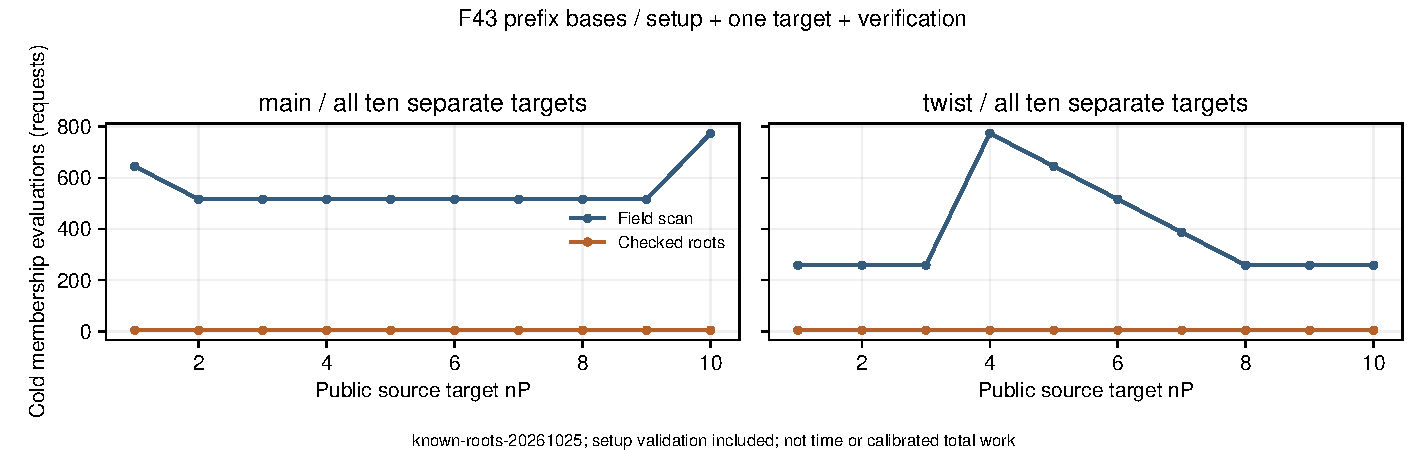
\includegraphics[width=\linewidth]{membership.pdf}

\noindent The 32 components have distinct, sometimes nested units. Sorting,
field tables, hashing, allocation, traversal, internal exponentiation and audit
remain unpriced. Matrix slots describe shape, not measured sparse allocation.
No time, calibrated total, GAE, $S$, rho or fastest-external claim is admitted.
This is a verified algorithm-request reduction; complete cost remains open.

\newpage
\section*{Completeness is proved, not inferred from zero tests}
For an integral domain, Lean proves
\[
  \prod_{a\in L}(x-a)=0\quad\Longleftrightarrow\quad x\in L.
\]
For two entries the polynomial is $x^2-(a+b)x+ab$. The constrained pair set is
exactly $\{a,b\}^2$ intersected with the remaining constraint $h(x,y)=0$.
The theorem does not need distinctness; this implementation needs it for an
ordered list without duplicates. The domain hypothesis is explicit.

The actual first-policy main membership is $x^2-17x+9$ with roots $4,13$;
the twist's is $x^2-32x+40$ with roots $15,17$, in $\mathbf F_{43}$. Lean
instantiates both with the actual reduced S3 constraint for arbitrary target
abscissa $z$. Every other pair is covered by the generic result and independently
checked polynomial bindings.

\begin{center}\begin{tabular}{lp{0.60\linewidth}}\toprule
Claim & Declaration in \texttt{KnownRoots}\\\midrule
Complete product root set & \texttt{product\_root\_iff}\\
Expansion and two-root set & \texttt{expanded\_two\_factors}, \texttt{quadratic\_roots\_iff}\\
Constrained solution set & \texttt{constrained\_pairs\_iff}\\
Actual main/twist input & \texttt{main\_actual\_input}, \texttt{twist\_actual\_input}\\\bottomrule
\end{tabular}\end{center}
The unchanged scoped gate passes 182 public named theorems /238 audited
declarations, zero failing or extra trusted axioms. The seven new declarations
include six theorems and one generated definition helper. Only standard
propext, Classical.choice and Quot.sound occur. Certificate
\texttt{IDC1he9f02ada0008638c} checks the expansion polynomial at 32+16 native
points, with false identity/source rejection; it does not prove completeness
or the native algorithm.

\noindent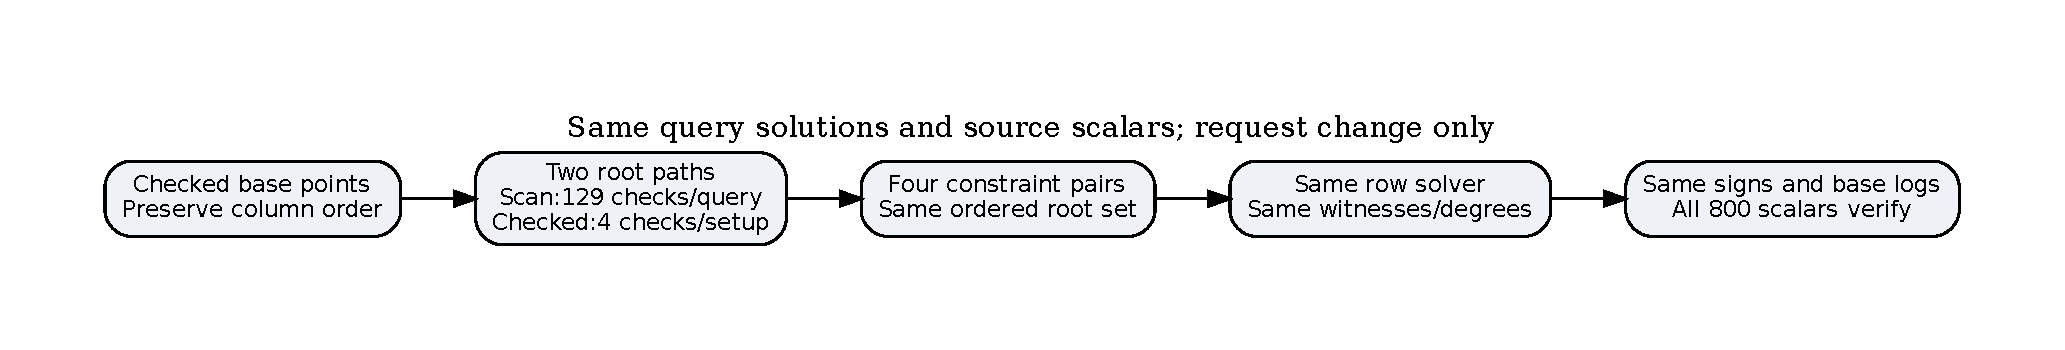
\includegraphics[width=\linewidth]{bridge.pdf}

\section*{Actual DLP, failures and limits}
Models \texttt{icv1-fp6-t0-74779950} and \texttt{icv1-fp6-t0-c6a8a47c} are
$E:y^2=x^3+x$ and $T:Y^2=X^3+4X$ over F43, order-11 generators $(31,18)$
and $(24,26)$. The existing actual map $(x,y)\mapsto(41x,11y)$ and checked
annihilator-aware recovery theorem bind the source DLP. This is an exceptional
base-field-isomorphic fixture, not a generic rational twist transfer.

Nine rehashed corruptions reject without receipt, including omitted/extra
roots, false membership and lost failed queries. The first run rejected a
wrong ascending-base assumption before accepting a case; the fixed protocol
preserves column order and sorts only query roots. Exact failures are retained.
The fresh replay and22 backend tests pass. The profile probe lacks gawk and
supplies no profile. Conductor remains unavailable, exit127.

Next test a setup-charged signed-base-point cache against this route, preserving
all lifts and scalars. General geometry, stationary yield, intrinsic regularity,
calibrated complete work, review, CI access and integration remain open.
Sources, full proof map, raw attempts, checks and reproduction are linked in
the accompanying README and versioned validation directory. No upload occurred.
\end{document}
